% a-project.tex, v-1.0.3 marcoreis baseado no
% abntex2-modelo-trabalho-academico.tex, v-1.9.7 laurocesar
% Copyright 2012-2018 by abnTeX2 group at http://www.abntex.net.br/ 
% 
% This work consists of the files 
% 
% -----------------------------------------------------------------------------
% Modelo para desenvolvimento de documentação de projetos acadêmicos
% (tese de doutorado, dissertação de mestrado e trabalhos de monografias em geral) 
% em conformidade com ABNT NBR 14724:2011: Informação e documentação. 
% -----------------------------------------------------------------------------
% Opções para a documentação
%
% Fancy page headings 
%\documentclass[fancyheadings, subook]{Classes/a-prj}
%\documentclass[fancyheadings, sureport]{Classes/a-prj}
%
% Fancy chapters and sections headings 
%\documentclass[fancychapter, subook]{Classes/a-prj}
%\documentclass[fancychapter, sureport]{Classes/a-prj}
%
% Fancy page , chapters and sections headings
%\documentclass[fancyheadings, fancychapter, subook]{Classes/a-prj}
\documentclass[fancyheadings, fancychapter, sureport]{Classes/a-report}
%
% -----------------------------------------------------------------------------
% Alguns comandos para a fancy page headings)
%
% Page header line width
%\footlinewidth{value}
%
% Page footer line width
%\headlinewidth{value}
%
% Page header and footer line width
%\headingslinewidth{value}
%
% Page header and footer lines without text
%\headingslinesonly
%
% The default line width is 0.3pt.
% Set the value to 0pt to remove the page header and/or footer line
%
% -------------------------------------------------------------------------------
% Formato de figuras suportado
% -------------------------------------------------------------------------------
% O formato das figuras depende da forma como o arquivo de saída é gerado.
% As figuras inseridas na pasta Figures serão automaticamente reconhecidas sem
% a necessidade de inserir a extensão do arquivo.
%
% O pdfLaTEX (PDF) suporta figuras com as extensões: pdf, jpg, png e mps.
%
% -------------------------------------------------------------------------------
% Árvore do diretório a-project.tex
%  Diretório
%       \Classes        (requerido)
%       \Figures        (requerido) --------------------------------->
%       \Figures\PDF    (optional)
%       \Figures\JPG    (optional) Figures located within these
%       \Figures\PNG    (optional) folders are searched automatically
%       \Figures\MPS    (optional)  by the a-prj class.
%       \Figures\EPS    (optional)
%       \Figures\PS     (optional) <--------------------------------
%       \Tables         (requerido)
%       \Others         (requerido)
%       \Chapters       (requerido)
%       \Appendices     (optional)
%       \References     (requerido)
%
% -------------------------------------------------------------------------------
% PDF File resumo
\ifpdf
    \hypersetup{
    	backref,
        colorlinks  = true,
        pdftitle    = Modelo de documentação,
        pdfauthor   = {Marco Reis, marco.a.reis@gmail.com},
        pdfsubject  = Mestre em Engenharia,
        pdfcreator  = Subtitulo,
        pdfproducer = PDFLatex,
        pdfkeywords = {documentação, latex, dissertação, tese}}
 \fi
%
% -------------------------------------------------------------------------------
% Relação de pacotes opcionais utilizados
\usepackage[utf8]{inputenc}
\usepackage[brazil]{babel}
\usepackage{longtable}
\usepackage{dcolumn}
\usepackage{multirow}
\usepackage{lscape}
%\usepackage{graphicx}
\usepackage{rotating}
%\usepackage{float,subfigure}
%\usepackage{graphicx, subfigure}
\usepackage{cite}
\usepackage[left=3cm,top=3cm,right=2cm,bottom=2cm]{geometry}
\usepackage[alf]{abntex2cite}
\usepackage{ifpdf}
\usepackage{shadow}
\usepackage{wrapfig}
\usepackage[normalem]{ulem}
\usepackage{makeidx}
\usepackage{yfonts}
\usepackage{algorithm}
\usepackage{algorithmic}
\usepackage{lmodern}
\usepackage[T1]{fontenc}
\usepackage{indentfirst}
\usepackage{color}
\usepackage{microtype}
\usepackage{lipsum}
\usepackage{caption}
\usepackage{subcaption}
\usepackage{ragged2e}
\usepackage{pdfpages}
\justifying
%
\makeindex 
\setlength{\LTcapwidth}{\textwidth}
%
\newtheorem{theorem}{Teorema}
\newtheorem{definition}[theorem]{Definição}
%
% -------------------------------------------------------------------------------
% Configurações do pacote backref
\renewcommand{\backrefpagesname}{Citado na(s) página(s):~}
% Texto padrão antes do número das páginas
\renewcommand{\backref}{}
% Define os textos da citação
\renewcommand*{\backrefalt}[4]{
	\ifcase #1 %
		Nenhuma citação no texto.%
	\or
		Citado na página #2.%
	\else
		Citado #1 vezes nas páginas #2.%
	\fi
}
% 
% -------------------------------------------------------------------------------
% Início do documento raiz
\begin{document}
% Definição do título da página
    \university{Centro Universitário SENAI CIMATEC}
	%\faculty{Programa de...}
	%\school{Escola de...}
% 
    %\course{Engenharia Elétrica}
    \typework{Relatório Parcial}
% 
	%\course{Mestrado em Modelagem Computacional e Tecnologia Industrial}
	%\typework{Disserta\c{c}\~ao de mestrado}
	%\typework{Exame de Qualificação de Mestrado}
% 
	%\course{Engenharia Elétrica}
	%\typework{Tese de doutorado}
	%\typework{Exame de Qualificação de doutorado}
%
% -------------------------------------------------------------------------------
% Informações gerais
    \thesistitle{Estudo do Estado da Arte sobre robôs antropormóficos}
    \hidevolume
    \thesisvolume{Volume 1 of 1}
    \thesisauthor{Juliana Maria S. de Santana}
    % \thesisauthorr{}
    \thesisadvisor{Prof. Marco Reis, M.Eng.}
    %\hidecoadvisor
    %\thesiscoadvisor{Marco Reis}
    \thesismonthyear{Novembro de 2021}
% 
    \maketitlepage
%
% ----------------------------------------------------------------------------
% Inserir Folha de rosto, Nota de estilo, folha de assinaturas, dedicatoria
    \begin{folharosto}

\begin{center}
\theauthor \\
% \theauthorr \\
%\theauthorrr \\
%\theauthorrrr \\
%\theauthorrrrr \\
\end{center}
\ \\
\ \\
\ \\
\ \\
\ \\
\begin{spacing}{2}
   \begin{center}
   {\LARGE {\bf \thetitle}}
   \end{center}
\end{spacing}
\ \\
\ \\
\ \\
\vspace*{85mm}
% \begin{flushright}

%    \begin{list}{}{
%       \setlength{\leftmargin}{7.5cm}
%       \setlength{\rightmargin}{0cm}
%       \setlength{\labelwidth}{0pt}
%       \setlength{\labelsep}{\leftmargin}}

%       \item \thetypework apresentada ao \thefaculty, Curso de \thecourse
%       do \theuniversity, como requisito parcial para a obten\c{c}\~ao do
%       t\'itulo de {\bf \thedegreetitle}.

%       \begin{list}{}{
%       \setlength{\leftmargin}{0cm}
%       \setlength{\rightmargin}{0cm}
%       \setlength{\labelwidth}{0pt}
%       \setlength{\labelsep}{\leftmargin}}

%       \item \'Area de conhecimento: Interdisciplinar

%       \item Orientador: \theadvisor
%       \newline \hspace*{2.1cm}  %{\it \theuniversity}

%       \end{list}
%    \end{list}

% \end{flushright}
\ \\
\ \\
\ \\
\ \\
%\begin{spacing}{1.5}
   \begin{center}
   Salvador \par
   \theuniversity \par
   2021
   \end{center}
%\end{spacing}

\end{folharosto}

    %\begin{notaestilo}
Esta \thetypeworkthree foi elaborada considerando as normas de
estilo (i.e. est\'eticas e estruturais) propostas aprovadas pelo
colegiado do \thefacultytwo e est\~ao dispon\'iveis em formato
eletr\^onico ({\it download} na P\'agina Web
http:$//$ead.fieb.org.br$/$portal\_faculdades$/$dissertacoes-e-teses-mcti.html
ou solicita\c{c}\~ao via e-mail \`a secretaria do
programa) e em formato impresso somente para consulta. \\

Ressalta-se que o formato proposto considera diversos itens das
normas da Associa\c{c}\~ao Brasileira de Normas T\'ecnicas (ABNT),
entretanto opta-se, em alguns aspectos, seguir um estilo pr\'oprio
elaborado e amadurecido pelos professores do programa de
p\'os-gradua\c{c}\~ao supracitado.

\end{notaestilo}

    %\begin{folhaassinaturas}

%\thispagestyle{empty}

\def\signature#1#2{\parbox[b]{1in}{\smash{#1}\vskip12pt}
\hfill \parbox[t]{3in}{\shortstack{\vrule width 3in height
0.4pt\\\small#2}}}

\def\InstituicaoMembro#1#2{\parbox[b]{1in}{\smash{#1}\vskip12pt}
\hfill \parbox[t]{3in}{\shortstack{\vrule width 3in \\\small#2}}}

\def\signaturepage{%

    \begin{spacing}{1.5}
        \begin{center}
        {\LARGE \theuniversity} \\
        {\large \thefaculty} \\
        {\large \thecourse} \\
        \end{center}
    \end{spacing}

   \vskip 0.25in plus 0.4in minus 0.1in

    \begin{spacing}{1.5}
        \begin{sloppypar}
        A Banca Examinadora, constitu\'ida pelos professores abaixo
        listados, leram e recomendam a aprova\c{c}\~ao [com distin\c{c}\~ao] da
        \thetypeworktwo, intitulada ``\thetitle",
        apresentada no dia (dia) de (m\^es) de (ano), como requisito
        parcial para a obten\c{c}\~ao do t\'itulo de {\bf \thedegreetitle}.\\
        \end{sloppypar}
    \end{spacing}

    \def\sigskip{\vskip0.15in plus 0.2in minus 0.1in}
    \def\beginskip{\vskip0.3875in plus 0.2in minus 0.1in}

    \beginskip
    \signature{Orientador:}{Prof. Dr. \theadvisor} \\
    \InstituicaoMembro{}{\theuniversity} \\

    \sigskip
    \beginskip
    \signature{Membro externo da Banca:}{Prof. Dr. Nome completo} \\
    \InstituicaoMembro{}{Institui\c{c}\~ao do membro da banca} \\

    \sigskip
    \beginskip
    \signature{Membro externo da Banca:}{Prof. Dr. Nome completo} \\
    \InstituicaoMembro{}{Institui\c{c}\~ao do membro da banca} \\

    %\sigskip
    %\beginskip
   % \signature{Membro interno da Banca:}{Prof. Dr. Nome completo} \\
   % \InstituicaoMembro{}{Institui��o do membro da banca} \\

    \vfill
    \newpage
    \setcounter{page}{3}
}
%*********************************************************************


\signaturepage


\end{folhaassinaturas}

    %\include{Others/dedicatoria}
    %\include{Others/agradecimentos}
%
% ----------------------------------------------------------------------------
% Resumo/abstract, sumário e siglas
    \begin{romanpagenumbers}
        \begin{thesisresumo}
Escreva aqui o resumo da disserta\c{c}\~ao, incluindo os contextos geral e espec\'ifico, dentro dos quais a pesquisa foi realizada, o objetivo da pesquisa, assun\c{c}\~ao filos\'ofica, os m\'etodos de pesquisa usados e as poss\'iveis contribui\c{c}\~oes que o que \'e proposto pode trazer \`a sociedade.

\ \\

% use de três a cinco palavras-chave

\textbf{Palavras-chave}: Palavra-chave 1, Palavra-chave 2, Palavra-chave 3, Palavra-chave 4, Palavra-chave 5

\end{thesisresumo}

        \begin{thesisabastract}
Escreva aqui, em ingl\^es, o resumo da disserta\c{c}\~ao, incluindo os contextos geral e espec\'ifico, dentro dos quais a pesquisa foi realizada, o objetivo da pesquisa, assun\c{c}\~ao filos\'ofica, os m\'etodos de pesquisa usados e as poss\'iveis contribui\c{c}\~oes que o que \'e proposto pode trazer \`a sociedade. 

\ \\

% use de tr�s a cinco palavras-chave

\textbf{Keywords}: Keyword 1, Keyword 2, Keyword 3, Keyword 4, Keyword 5

\end{thesisabastract}

        % Make list of contents, tables and figures
        \thesiscontents
        %\pdfbookmark[1]{Lista de Tabelas}{lot} \listoftables
        %\newpage
        %Include other required section
        %\begin{thesisabbreviations}
\begin{footnotesize}
\begin{longtable}[l]{p{2cm}l}
  tprax   \dotfill & \thefaculty \\
  WWW       \dotfill &  World Wide Web \\
\end{longtable}
\end{footnotesize}
\end{thesisabbreviations}

        %\begin{thesissymbols}
\begin{footnotesize}
\begin{longtable}[l]{p{2cm}l}
  $\partial$   \dotfill  & Bla bla bla \\
  $\prod$       \dotfill & ble ble ble \\
  $\partial$   \dotfill  & Bla bla bla \\
  $\prod$       \dotfill & ble ble ble \\
  $\partial$   \dotfill  & Bla bla bla \\
  $\prod$       \dotfill & ble ble ble \\
  $\partial$   \dotfill  & Bla bla bla \\
  $\prod$       \dotfill & ble ble ble \\
  $\partial$   \dotfill  & Bla bla bla \\
  $\prod$       \dotfill & ble ble ble \\
  $\partial$   \dotfill  & Bla bla bla \\
  $\prod$       \dotfill & ble ble ble \\
  $\partial$   \dotfill  & Bla bla bla \\
  $\prod$       \dotfill & ble ble ble \\
  $\partial$   \dotfill  & Bla bla bla \\
  $\prod$       \dotfill & ble ble ble \\
  $\partial$   \dotfill  & Bla bla bla \\
  $\prod$       \dotfill & ble ble ble \\
  $\partial$   \dotfill  & Bla bla bla \\
  $\prod$       \dotfill & ble ble ble \\
  $\partial$   \dotfill  & Bla bla bla \\
  $\prod$       \dotfill & ble ble ble \\
  $\partial$   \dotfill  & Bla bla bla \\
  $\prod$       \dotfill & ble ble ble \\
  $\partial$   \dotfill  & Bla bla bla \\
  $\prod$       \dotfill & ble ble ble \\
  $\partial$   \dotfill  & Bla bla bla \\
  $\prod$       \dotfill & ble ble ble \\
  $\partial$   \dotfill  & Bla bla bla \\
  $\prod$       \dotfill & ble ble ble \\
  $\partial$   \dotfill  & Bla bla bla \\
  $\prod$       \dotfill & ble ble ble \\
  $\partial$   \dotfill  & Bla bla bla \\
  $\prod$       \dotfill & ble ble ble \\
  $\partial$   \dotfill  & Bla bla bla \\
  $\prod$       \dotfill & ble ble ble \\
  $\partial$   \dotfill  & Bla bla bla \\
  $\prod$       \dotfill & ble ble ble \\          
\end{longtable}
\end{footnotesize}
\end{thesissymbols}

        %Switch the page numbering back to the default format
    \end{romanpagenumbers}
%
% ---------------------------------------------------------------------------
% Include thesis chapters
    \parskip=\baselineskip
    % \chapter{Introdução}
\label{chap:intro}

Um dos principais objetivoss robôs móveis têm a capacidade de se moverem sob seu próprio controle. Quando o robô é capaz de executar tarefas usando estado físico e/ou sensores sem intervenção humana é categorizado como autônomo, conforme às definições da norma \cite{ISO}. De acordo com \citeonline{Rubio} plataformas móveis podem ser classificados, quanto ao sistema de locomoção, como terrestres, aquáticos e aéreos. Os terrestres são subdivididos em robôs que possuem rodas, pernas (bípedes) ou esteiras. Cada um desses métodos possuem características especifícas quanto ao movimento a ser realizado. Os bípedes, por exemplo, simulam um caminhar antropomórfico, semelhante aos humanos. 

De acordo com \citeonline{He2020}, mais de 50\% da superfície terrestre é inacessível por veículos tradicionais com rodas e trilhas. Enquanto, robôs com pernas possuem uma maior mobilidade em ambientes irregulares porém, eles possuem mecânismos e modos de controle muito mais complexos.\cite{Wieber20161203}

Segundo \citeonline{He2020} a perfomance de robôs com pernas estão relacionados com vários fatores, incluindo seus mecânismos e atuação, percepção, e métodos de controle. Por isso, é necessário realizar uma pesquisa sobre a evolução dessas tecnologias.

O desenvolvimento desta documentação consiste na análise dos robôs humanóides tendo como base alguns dos principais artigos relacionados ao seu estudo assim como informações disponibilizadas pelos desenvolvedores, destacando suas principais caracteristicas físicas como tipos de sensores utilizados pelo sistema de percepção e estratégias de design mecânico e também informações relacionadas ao sistema de controle.

\section{Objetivo}
\label{sec:obj}

O estudo bibliográfico foi realizado com o intuito de auxiliar no desenvolvimento do projeto Walker que tem como objetivo construir um robô humanóide autônomo de pequeno porte. Esta pesquisa visa contribuir com informações obtidas através das análise das principais características dos sistemas dos robôs humanoídes já existentes. 

\section{Justificativa}
\label{sec:justi}

Robôs antropomórficos são amplamente utilizados em diversas áreas no dia-a-dia, desde interações com humanos até aplicações na área da saúde, bem como em pesquisas acadêmicas, sendo uma configuração mais adequada para transposição de ambientes de difícil navegação.

\citeonline{Gupta2017607} destaca que a vantagem da locomoção por pernas é a utilização de passos discretos para o equilibrio e a movimentação do robô, o que permite que este realize manobras em terrenos acidentados e escadas. E, dentre os robôs com pernas, os robôs bípedes oferecem outras vantagens como mãos livres para manipulação, locomoção com maior eficiência energética e a capacidade de torcer os pés para rotacionar em torno do eixo logintudinal do seu próprio corpo.

Uma abordagem trazida por \citeonline{Joseph2018} aponta a aplicação dos robôs humanóides para auxiliar cuidadores e pacientes, especialmente em áreas de risco, como ambientes contaminados. Podendo ser utilizados para usos médicos e cirúrgicos, para dar assistência aos pacientes e cuidadores e também para a área de segurança.

Segundo \citeonline{Chatterjee2017603} os robôs humanóides são vantajosos para serem aplicados em atividades domésticas, podendo ajudar no cuidado de idosos, podem ser uma fonte de entretenimento, além de realizar as tarefas domésticas.

Além disso, faz-se necessário o formento ao desenvolvimento da Robótica no estado da Bahia, bem como o estudo de robôs antropomórficos dentro da Instituição Senai Cimatec, elevando seu nível competitivo.


%*******************************************************************

% \chapter{Ambiente de desenvolvimento}
% \label{chap:fund}


% \section{Ambiente de aplicação}
% \label{sec:fun1}

% \section{Situação atual no desenvolvimento de Robôs Bípedes}
% \label{sec:fun2}

% \section{Mercado de atuação}
% \label{sec:fun3}

%*******************************************************************

\chapter{Metodologia}
\label{chap:metod}

Para o desenvolvimento deste estudo do Estado da Arte dos robôs antropormóficos foi utilizada a metodologia do método BILI (Bibliographic and Literary Review Method), a qual será explicada nos tópicos seguintes.

\section{Método bili}
\label{sec:bili}

O método BILI (Bibliographic and Literary Review Method) é uma metodologia de pesquisa para o estudo das revisões bibliográficas que visa otimizar a busca e a seleção das referências. Este método é composto por quatro fases e utiliza  ferramentas como o  Rstudio, o Cmaptools e o Mendeley para a seleção, revisão e organização das documentações encontradas. Através desta metodologia é possível encontrar os artigos e autores mais relevantes para a pesquisa.

\begin{figure} [H]	
    \centering
    \caption{Fases do método BILI}
    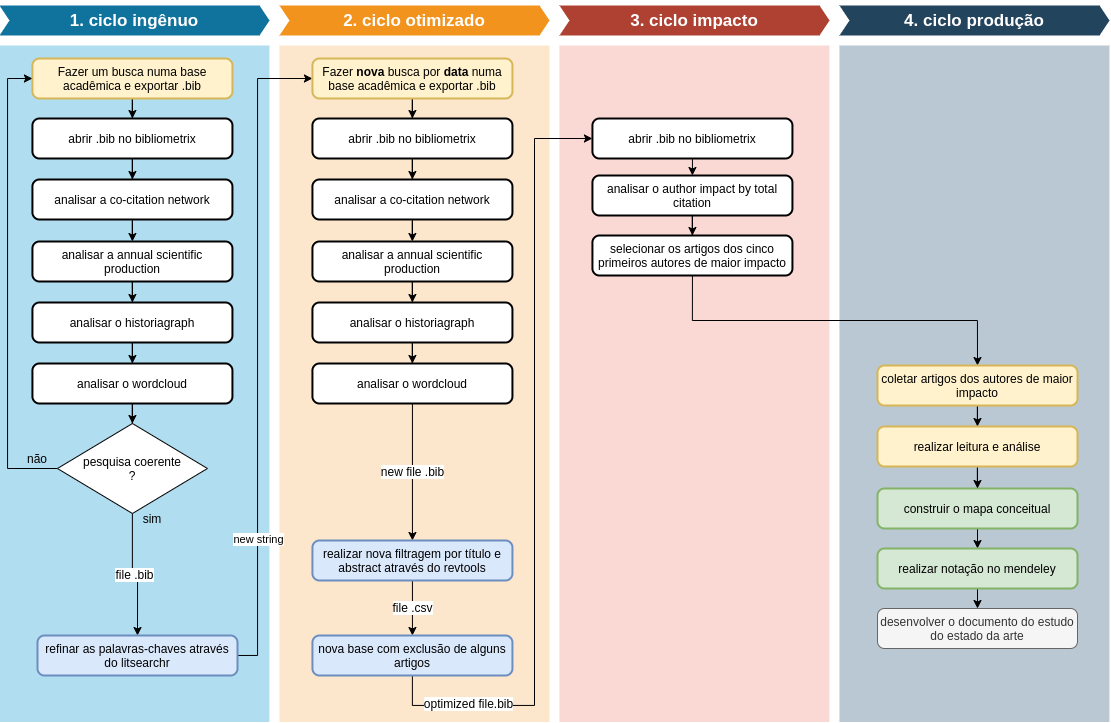
\includegraphics[width=0.6\textwidth]{bili}
    % \caption*{Fonte: Autoria própria.}
    \label{fig:bili}
\end{figure}

\subsection{Fase 1}
\label{sec:fase1}

A primeira fase é denominada de ciclo ingênuo e corresponde a pesquisa inicial feita em uma base acadêmica  de onde é exportado o arquivo .bib. Através deste arquivo utilizando a ferramenta biblioshiny, fornecida pelo pacote Bibliometrix, é feita uma análise da rede de co-citação, da produção cientifica anual e das palavras que aparecem com maior frequência nos artigos. Caso estas informações estejam coerentes com a pesquisa desejada, o pacote litsearchr é utilizado para auxiliar no refinamento da pesquisa através das palavras-chaves. Se o resultado obtido não for satisfatório a busca na base acadêmica deve ser refeita. E, por fim, é gerada uma nova string que será utilizada para realizar uma nova busca. 


\subsection{Fase 2}
\label{sec:fase2}

A fase dois é chamada de ciclo otimizado pois, nesta fase é feita uma nova busca na base acadêmica porém, utilizando as palavras-chaves refinadas. Desta forma, o passo seguinte é realizar a mesma análise feita no primeiro ciclo e, após está análise é feita uma filtragem dos artigos utilizando o Revtools. Esta ferramenta permite o pesquisador selecionar os melhores artigos para sua pesquisa através da leitura dos títulos e abstracts. E, então é exportado um novo arquivo .bib com os dados otimizados para a pesquisa. 

\subsection{Fase 3}
\label{sec:fase3}

Na terceira fase, denominada ciclo impacto, é feita a análise do imapcto do autor utilizando o bibliometrix. E, então são selecionados os artigos dos cinco primeiros autores de maior impacto.

\subsection{Fase 4}
\label{sec:fase4}

Na última fase, chamada de ciclo produção, é feita a leitura e análise dos artigos selecionados no ciclo anterior e então foi construido um mapa conceitual sobre a pesquisa assim como, todos os artigos selecionados foram armazenados no Mendeley, onde também foram feitas algumas anotações. E, por fim, foi desenvolvida esta documentação com base nestas análises.


\section{Construção do relatório}
\label{sec:const}

%*******************************************************************

\chapter{Estudo do estado da arte}
\label{chap:sota}

\section{Robôs Antropormóficos}
\label{ssec:robos}

Robôs antropormóficos, também conhecidos como humanóides, possuem uma estrutura baseada no corpo humano, com  membros e movimentos que visam uma mobilidade que permita ao robô realizar tarefas diversificadas, principalmente para auxiliar as pessoas em atividades diarias, para o entretenimento e realizar tarefas de risco.

De acordo com \citeonline{Li20211} em comparação com outros tipos de robôs, os humanóides são mais adaptaveis ao ambiente e possuem uma boa habilidade para evitar obstáculos, por isso atraem a atenção de muitos pesquisadores.

Estes movimentam-se e ajustam o seu equilibrio por meio das suas duas pernas, inclusive em terrenos irregulares. Sendo a habilidade de andar com um bom equilibrio a sua habilidade mais básica.

Para ter uma boa mobilidade e ser capaz de realizar as tarefas proposta o robô deve possuir uma locomoção rápida e estável sendo este um dos desafios na implementação deste tipo de robô. O gerador de trajetórias e o controlador são projetados visando uma locomoção rápida, flexível e robusta sendo estes os grandes desafios desta área, sendo algumas das principais áreas de estudo.

\subsection{Definição}
\label{ssec:defi}

Os robôs antropormóficos, também conhecidos como humanóides, são robôs que possuem atributos semelhantes a forma humana como cabeça, braços e pernas. São robôs bípedes, ou seja, que se locomovem sobre os dois pés.

\subsection{Componentes principais}
\label{ssec:comp}

A percepção visual é fundamental para a maioria dos sistemas autonomos que operam em ambientes repletos de obstáculos e para realizar uma série de tarefas essenciais como interagir com o humano, manipular e rastrear objetos. \cite{Joseph2018} 

\citeonline{Chatterjee2017603} aponta que os robôs domésticos utilizam da Inteligência Artificial para possuir habilidades como reconhecimento de voz, reconhecimento facial humano, emoção, entre outros.

Para permitir que o robô alcance uma locomoção estável e rápida deve-se atentar-se ao projeto da estrutura cinemática do robô e a alguns objetivos do design para melhorar a dinâmica dos membros do robô.\cite{Buschmann2009141}



\subsection{Tabela Comparativa}
\label{ssec:tabela}





%******************************************************************


\section{Revisão bibliográfica}
\label{sec:biblio}

\subsection{Rede de citação}
\label{ssec:rede}

\subsection{Principais autores}
\label{ssec:autor}

%******************************************************************

\section{Modelos de robôs bípedes}
\label{sec:modelos}

Nesta seção serão abordadas as principais características de alguns modelos de robôs humanoídes comumente utilizados por pesquisadores para realizar estudos sobre a locomoção bípede.

Um robô terrestre que se locomove sobre dois pés é classificado como bípede. Para isto, os movimentos realizados por este robô são similares a um andar antropomórfico. Movimentos antropomórficos são amplamente estudados e utilizados tanto na área de robótica voltada à saúde, como na industrial

\subsection{Robô NAO}
\label{ssec:nao}

O NAO é um robô desenvolvido pela SoftBank Robotics muito utilizado para pesquisas e educação. Originalmente, ele foi criado pela Aldebaran Robotics para ser um companheiro doméstico. Dentre as suas principais aplicações estão a sua utilização como assistentes em empresas e institutos de saúde.Este robô utiliza um frameqork específico conhecido como NAOqios, o qual utiliza Python ou C++.  

O NAO possui 58cm de altura, duas câmera 2D para reconhecer objetos e pessoas, é capaz de se comunicar em diversas línguas por meio dos seus quatro microfones e speakers. O robô também dispõe de sete sensores de toque localizados na sua cabeça, nas suas mãos e pés, sonares e uma IMU para reconhecer seu ambiente e se localizar no espaço. Ele apresenta um total de 25 graus de liberdade o que permite que ele se movimente e se adapte no ambiente.

\begin{figure} [H]	
    \centering
    \caption{Robô NAO}
    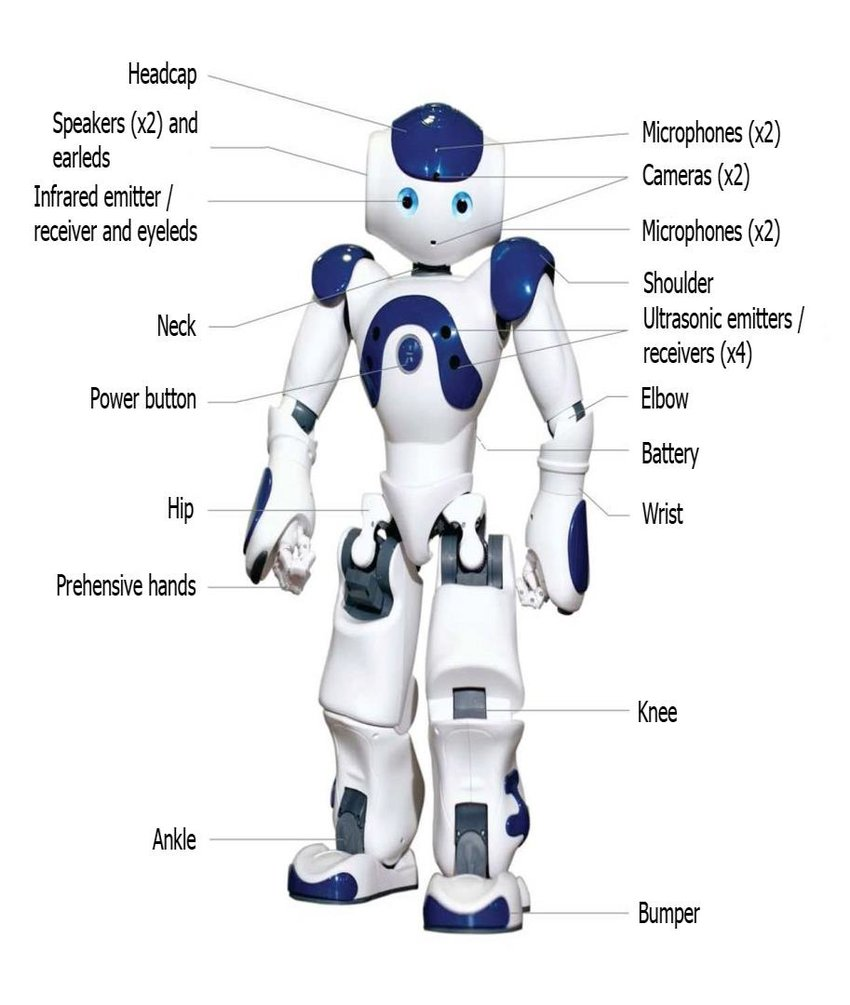
\includegraphics[width=0.6\textwidth]{nao}
    % \caption*{Fonte: Autoria própria.}
    \label{fig:nao}
\end{figure}

\subsection{Robô DARWIN-OP}
\label{ssec:darwin}

O Darwin-OP (Dynamic Anthropomorphic Robot with Intelligence-Open Platform)  é um pequeno humanoide desenvolvido pela Robotis. Ele tem 20 graus de liberdade e pesa 2.9kg, possui uma camera HD, giroscópio, acelerômetro e um microfone stereo. O Darwin é capaz de andar, falar e dançar sendo bastante utilizado por pesquisadores e programadores.

\begin{figure} [H]
    \centering
    \caption{Robô Darwin-OP}
    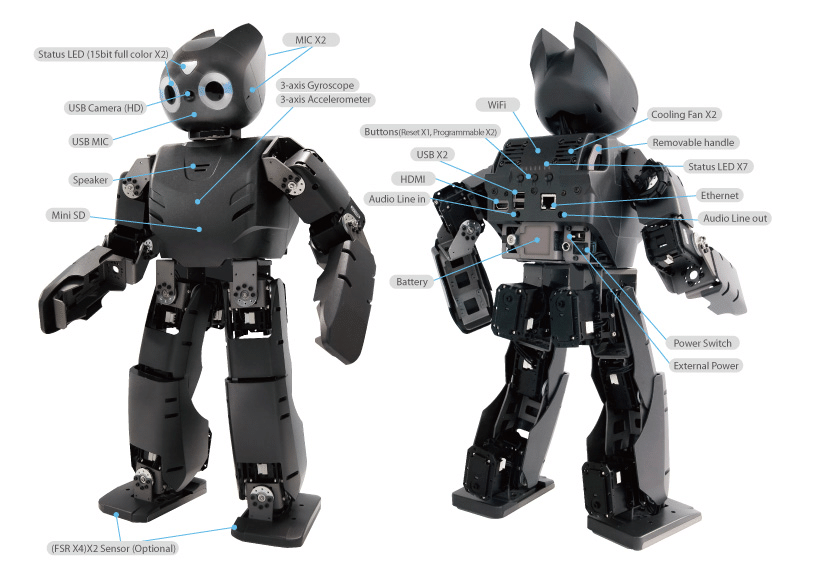
\includegraphics[width=0.8\textwidth]{darwin}
    % \caption*{Fonte: Autoria própria.}
    \label{fig:darwin}
\end{figure}

\subsection{Robô LOLA}
\label{ssec:lola}

O Lola é um robô humanoide desenvolvido na Universidade Tecnica de Munich (TUM) e financiado pela Funfação de pesquisa alem (DFG), utilizado em pesquisas sobre a dinâmica e aspectos de controle da locomoção bípede. A versão do Lola apresentada na figura X possui 24 graus de liberdade, uma altura de 180cm e pesa aproximadamente 60kg. O seu design foi projetado para possuir pouco peso, uma regidez efetiva alta, pernas com uma inércia baixa e o centro de gravidade alto. Com relação aos sensores utilizados pelo robô, o Lola possui enconders nos eixos dos seus motores e sensores de força/torque (FTS) customizados em seus pés, apresenta uma IMU em seu torso e uma câmera Intel RealSense em sua cabeça. É um robô versátil, com um design projetado para demonstrar uma caminhada bípede rápida.

\begin{figure} [H]
    \centering
    \caption{Robô LOLA}
    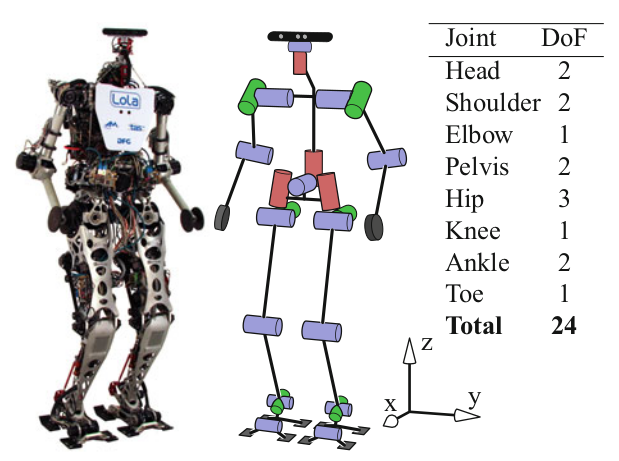
\includegraphics[width=0.8\textwidth]{lola}
    % \caption*{Fonte: Autoria própria.}
    \label{fig:lola}
\end{figure}

\subsection{Robô HUBO 2}
\label{ssec:hubo}

O HUBO 2 foi desenvolvido no laboratório HUBO no KAIST (Korean Advanced Institute os Science and Technology), na Coréia do Sul. Ele possui 125cm, pesa 45kg e possui 40 graus de liberdade. O seu design tinha como objetivo ser bem leve, o que permitiu que o HUBO 2 fosse capaz de correr em uma velocidade de 3.6 km/h. O seu sistema de percepção é composto por câmeras, sensores de inércia, inclinação e  força/torque. O seu grande diferencial em relação a outros robôs bípedes é a capacidade de utilizar uma marcha com pernas esticadas.

\begin{figure} [H]
    \centering
    \caption{Robô HUBO 2}
    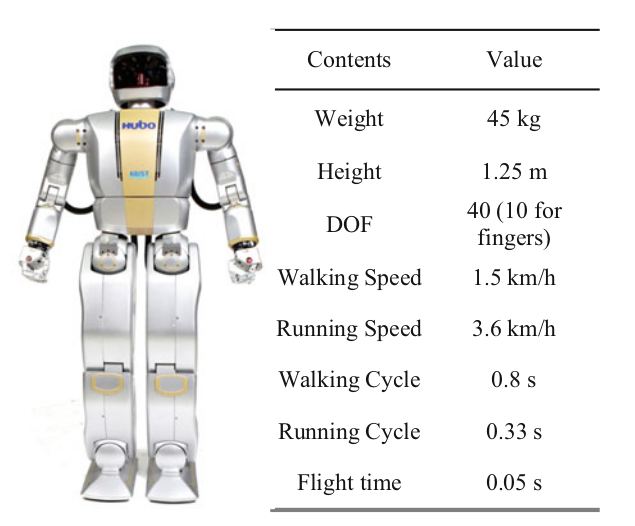
\includegraphics[width=0.8\textwidth]{hubo2}
    % \caption*{Fonte: Autoria própria.}
    \label{fig:hubo2}
\end{figure}


\section{Estudo das funcionalidades e mecânismos}
\label{sec:robos}

Nesta seção serão apresentadas as principais caracteristicas dos sistemas de percepção e controle dos robôs antropormóficos, assim como da estrutura mecânica destes robôs. Estes são quesitos de extrema importância no desenvolvimento destes robôs pois influênciam na eficiência do seu sistema.

These strategies can be easily combined with a visionsystem  to  navigate  obstacle-free,  flat  regions  [11].  Mostare  based  on  a  vision  system  that  can  recognize  walkablesurfaces  in  the  environment;  these  are  sent  to  the  walkingcontrol  system,  which  adapts  footstep  locations  and  robottrajectories to navigate over these surface model (Modifying the Estimated Ground Height to Mitigate Error Effects onBipedal Robot Walking)

\subsection{Percepção}
\label{ssec:percepcao}

Os sensores comumente usados nos robôs humanóides podem ser classificados em dois grupos, os sensores proprioceptivos são utilizados para medir os estados de cada junta e do corpo do robô e os sensores exteroceptivos utilizados para obter informações do ambiente. São utilizados sensores internos para medir o estado do robô, como ângulos, velocidades e torques das juntas. Para detectar informações da postura do robô, utiliza-se os sensores IMU, incluindo acelerômetros e giroscópios. Enquanto, a interação entre o robô e o ambiente podem ser detectados por meio de sensores táteis e de força/torque. E, as câmeras e sensores de alcance medem e estimam as informações do ambiente ao redor do robô. 

\begin{figure} [H]
    \centering
    \caption{Classificação dos sensores}
    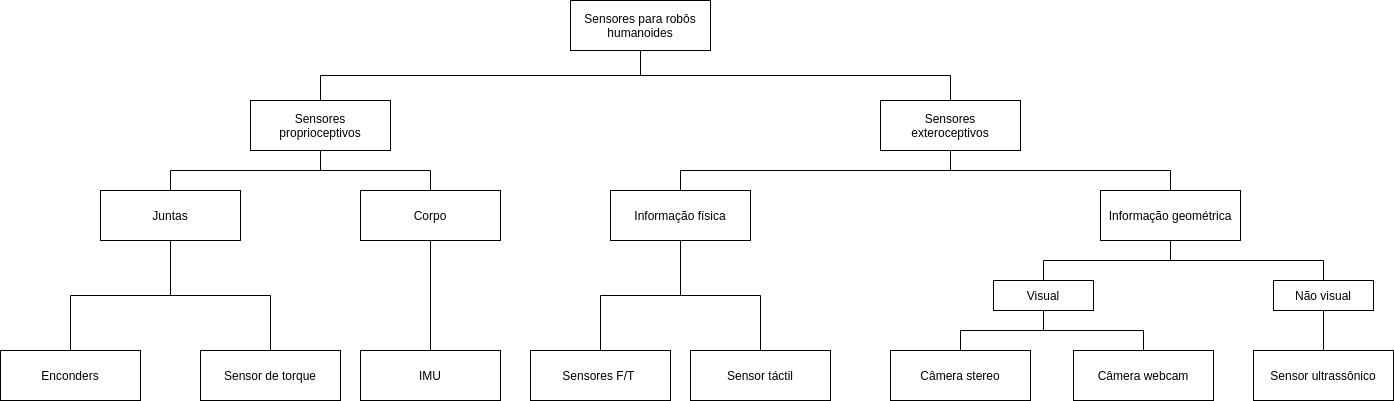
\includegraphics[width=0.8\textwidth]{sensores}
    % \caption*{Fonte: Autoria própria.}
    \label{fig:sensors}
\end{figure}

Segundo \citeonline{Buschmann2009141} o sistema de sensores do LOLA é otimizado para qualidade de sinal e largura de banda. Sensores angulares absolutos nos eixos de saída de todas as juntas compensam as elasticidades e não linearidades nos trens de força e permitem que o robô (teoricamente) comece a partir de posições arbitrárias. Dois sensores de força / torque de seis eixos feitos sob medida são fortemente integrados à estrutura do pé. Um erro de calibração de menos de 0,5 é obtido aplicando muitos casos de carga diferentes. Com um peso total de 395 g, o sensor inclui uma proteção contra sobrecarga e todos os componentes eletrônicos necessários. A unidade de medição inercial (IMU) estima a orientação e as velocidades angulares da parte superior do corpo. Visto que a precisão e a qualidade do sinal do IMU afetam consideravelmente o desempenho do controlador de estabilização, escolhemos IMU de alta precisão com giroscópios de fibra ótica e acelerômetros MEMS.

No projeto desevolvido por \citeonline{Kien2017} quatro sensores ultrassônicos, dois em cada perna, são usados para feedback da posição para caminhar e girar. O acelerômetro é usado para medir o ângulo de inclinação e para detectar a queda instantânea do robô. Sensores Resistivos de Força (FSR) são usados para determinar o centro de pressão (COP) que por sua vez é usado para calcular o ZMP do robô.


\subsection{Mecânismos}
\label{ssec:mec}

Um robô humanóide tem o formato do corpo semelhante ao de um corpo humano e tem como base a literatura sobre a análise e coordenação da marcha humana. Eles possuem um grande número de graus de liberdade (DOF), para serem capazes de realizar um movimento bípede semelhante ao humano. Para que este movimento seja mais natural e flexível, segundo \citeonline{Buschmann2009141}, recomenda-se considerar uma configuração redundante com DOFs adicionais.

Para melhorar a dinâmica das pernas do robô deve-se garantir uma regidez mecânica suficiente, centro de massa alto e baixos momentos de inércia dos elos das pernas.

O objetivo básico do projeto , é, portanto, equilibrar a rigidez estrutural e o desempenho do atuador com a leveza dos componentes mecânicos.
A estrutura mecânica do Lola, por exemplo, é caracterizado pelo design leve e consistente com alta rigidez efetiva.

São utilizados servo atuadores leves e a inércia resultante das pernas é minimizada por um design sofisticado da estrutura e mecanismos de acionamento, resultando em um comportamento de aceleração superior.

\subsection{Controle}
\label{ssec:control}

A figura \ref{fig:steps-control} ilustra os passos necessários para o controle da caminhada de um robô humanóide, onde a primeira etapa deste processo é o planejamento dos passos o qual é feito através do ajuste de alguns parâmetros de forma que o robô realize os movimentos de acordo com as fases de suporte dos pés ilustradas na figura \ref{fig:support-phases}.


\begin{figure} [H]
    \centering
    \caption{Elementos para o desenvolvimento do controlador de caminhada}
    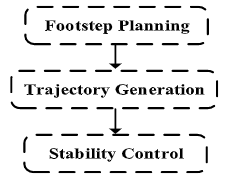
\includegraphics[width=0.8\textwidth]{walk-control}
    \caption*{Fonte: \cite{Kashyap2021306}.}
    \label{fig:steps-control}
\end{figure}


\begin{figure} [H]
    \centering
    \caption{Diferentes fases de suporte dos pés durante a locomoção de robôs humanóides}
    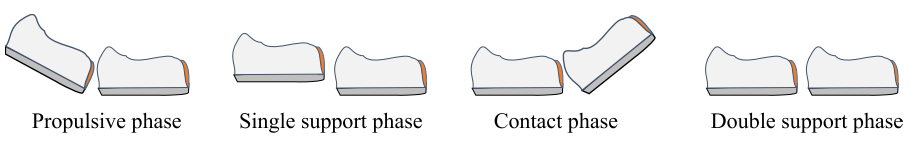
\includegraphics[width=0.8\textwidth]{support-phases}
    \caption*{Fonte: \cite{Kashyap2021306}.}
    \label{fig:support-phases}
\end{figure}

Existem basicamente dois tipos de marchas observadas em sistemas com pernas:  estaticamente estável e  dinâmicamente estável. Se o passo do robô permite que a projeção do seu centro de massa permaneça suficientemente dentro do polígono de suporte, projetado pelo pé do robô, entaão é estaticamente estável. Porém, se a projeção ocasionalmente sai do polígono de suporte , não deixando o robô cair ou tombar, então o sistema é dinâmicamente estável.

Existem quatro modelos que são frequentemente utilizados como representação aproximada do robô bípede. O Modelo do Pêndulo Invertido Linear (LIPM) considera que toda a massa do robô está concentrada em um ponto movendo-se em uma altura constante e assume que as pernas não possuem peso este modelo foi amplamente aplicado em diversas pesquisas como XXXX. Um outro modelo é o Pêndulo Invertido com Volante (IPF) que não considera que a altura é constante e adiciona um volante pata contabilizar o momento angular interno. O Pêndulo Invertido com Mola (SLIP) adiciona uma mola para modelar as pernas do robô como um pula-pula sem massa. E o Compass -Gait Biped (CG) que trata o robô como um pêndulo duplo com massas concentradas no centro de massa e nas pernas oscilantes.\cite{Grizzle20141955} Ao utilizar um modelo de robô reduzido,por exemplo, \cite{Wahrmann20171471} a estratégia no controle em tempo real tornando o robô mais robusto contra erros de percepção e de superfícies irregulares. 

Também é necessário implementar um gerador de trajetórias, o qual gera algum tipo de movimento considerando o deslocamento do Centro de Massa (COM) e do Ponto de Momento Zero (ZMP) assim como, a descrição da cinemática inversa. Desta forma, os ângulos das juntas do robô são obtidas. E, então é necessário um controlador para estabilizar estes ângulos nas juntas para garantir que o robô permanece em pé e realize todas as tarefas sem cair. \cite{Kashyap2021306}

\citeonline{Kasaei2018743} apresenta uma estrutura de um controlador com um loop fechado baseada no método Central Pattern Generator (CPG) que propõem um modelo de controle inspirado nas caracteristicas biológicas. Desta forma, este método tenta produzir um caminhar estável atravéz de padrões rítmicos em relação a movimentação dos seus membros. Este teste foi realizado em um robô NAO simulado com a proposta de gerar uma movimentação estável e rápida.

\begin{figure} [H]
    \centering
    \caption{Arquitetura geral do gerador de passos}
    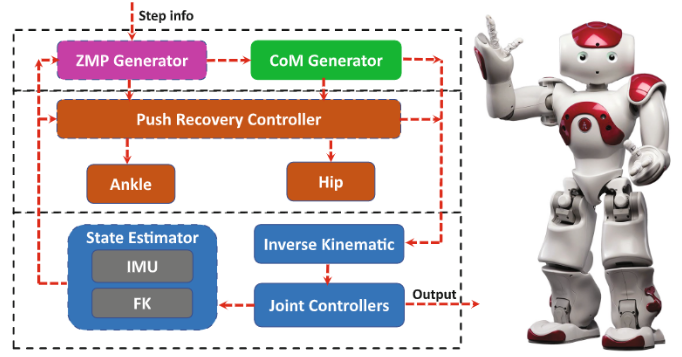
\includegraphics[width=0.8\textwidth]{arquiteturaNAO}
    \caption*{Fonte: \cite{Kasaei2018743}}
    \label{fig:arquitetura-nao}
\end{figure}

Em sua pesquisa \cite{Joe2019} implementa um framework de controle do equilíbrio que estabiliza os passos do robô em relação aos distúrbios. O controlador de equilíbrio é formado pelos controladores de orientação dos pés, comprimento da perna e ZMP. Estes testes foram realizados no robô DRC-HUBO+modificado. O framework proposto apresentou bons resultados permitindo que o robô se deslocasse de forma estável mantendo a postura desejada em terrenos irregulares.


\begin{figure} [H]
    \centering
    \caption{Visão geral do fluxo de informações do pramework de controle de equilíbrio proposta}
    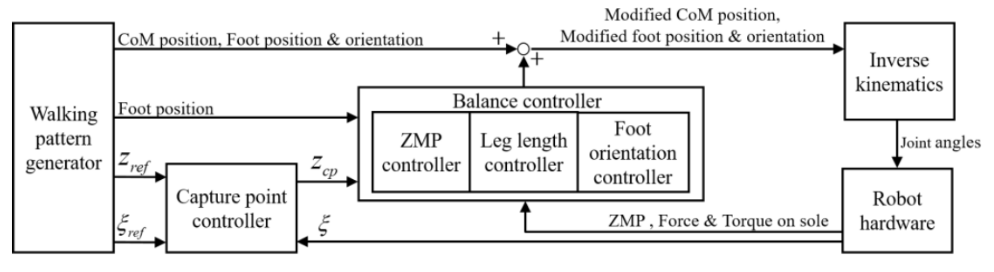
\includegraphics[width=0.8\textwidth]{controlador}
    \caption*{Fonte: \cite{Joe2019}}
    \label{fig:framework-control}
\end{figure}


O projeto de controle para sistemas subactuados são mais difícies devido a quantidade de graus de liberdades controláveis ser menor que a real quantidade de grau de liberdade do sistema. Em \cite{Gupta2017607} são abordadas outras estratégias de controle desenvolvidas para robôs subactuados como virtual constraints, HZD (Hybrid Zero Dynamics), Pointcaré map, etc.



%******************************************************************

\section{Mapa conceitual do estudo}
\label{sec:mapa}



%******************************************************************

\section{Organização e compartilhamento dos dados}
\label{sec:org}


%******************************************************************

\chapter{Conclusão}
\label{chap:conclu}


\section{Considerações finais}
\label{sec:consider}



These strategies can be easily combined with a visionsystem  to  navigate  obstacle-free,  flat  regions  [11].  Mostare  based  on  a  vision  system  that  can  recognize  walkablesurfaces  in  the  environment;  these  are  sent  to  the  walkingcontrol  system,  which  adapts  footstep  locations  and  robottrajectories to navigate over these surface model (Modifying the Estimated Ground Height to Mitigate Error Effects onBipedal Robot Walking)
    \chapter{Introdução}
\label{chap:intro}

De acordo com \citeonline{Rubio} plataformas móveis podem ser classificadas, quanto ao sistema de locomoção, como terrestres, aquáticos e aéreos. Os terrestres são subdivididos em robôs que possuem rodas, pernas (bípedes) ou esteiras, em que cada um  possui características específicas quanto ao movimento a ser realizado. Os bípedes, por exemplo, simulam um caminhar antropomórfico, semelhante aos humanos. 

De acordo com \citeonline{He2020}, mais de 50\% da superfície terrestre é inacessível por veículos tradicionais com rodas e trilhas. Enquanto, robôs com pernas possuem uma maior mobilidade em ambientes irregulares porém, eles possuem mecânismos e modos de controle muito mais complexos.\cite{Wieber20161203}

Segundo \citeonline{He2020} a perfomance de robôs com pernas esta relacionada com vários fatores, incluindo seus mecânismos, atuação, percepção, e métodos de controle. Por isso, é necessário realizar uma pesquisa sobre a evolução dessas tecnologias.

O desenvolvimento desta documentação consiste na análise dos robôs humanóides tendo como base alguns dos principais artigos relacionados ao seu estudo assim como informações disponibilizadas pelos desenvolvedores, destacando suas principais características físicas como tipos de sensores utilizados pelo sistema de percepção e estratégias de design mecânico e também informações relacionadas ao sistema de controle.

\section{Objetivo}
\label{sec:obj}

O estudo bibliográfico foi realizado com o intuito de auxiliar no desenvolvimento do projeto Walker que tem como objetivo construir um robô humanóide autônomo de pequeno porte. Esta pesquisa visa contribuir com informações obtidas através das análise das principais características dos sistemas dos robôs humanoídes já existentes. 

\section{Justificativa}
\label{sec:justi}

Robôs antropomórficos são amplamente utilizados em diversas áreas no dia-a-dia, desde interações com humanos até aplicações na área da saúde, bem como em pesquisas acadêmicas, sendo uma configuração mais adequada para transposição de ambientes de difícil navegação.

\citeonline{Gupta2017607} destacam que a vantagem da locomoção por pernas é a utilização de passos discretos para o equilíbrio e a movimentação do robô, o que permite que este realize manobras em terrenos acidentados e escadas. E, dentre os robôs com pernas, os robôs bípedes oferecem outras vantagens como mãos livres para manipulação, locomoção com maior eficiência energética e a capacidade de torcer os pés para rotacionar em torno do eixo logintudinal do seu próprio corpo.

Uma abordagem trazida por \citeonline{Joseph2018} aponta a aplicação dos robôs humanóides para auxiliar cuidadores e pacientes, especialmente em áreas de risco, como ambientes contaminados. Podendo ser utilizados para usos médicos e cirúrgicos, para dar assistência aos pacientes e cuidadores e também para a área de segurança.

E, segundo \citeonline{Chatterjee2017603} os robôs humanóides são vantajosos para serem aplicados em atividades domésticas, podendo ajudar no cuidado de idosos, podem ser uma fonte de entretenimento, além de realizar as tarefas domésticas.

    % \chapter{Conceito do projeto}
\label{chap:fundteor}
%--------- NEW SECTION ----------------------
Os robôs móveis têm a capacidade de se moverem sem a assistência de um operador humano. Os mesmos podem ser classificados,quanto ao sistema de locomoção, como terrestres, aquáticos e aéreos. Os terrestres são subdivididos em robôs que possuem rodas, pernas (bípedes) ou esteiras (ref:Review ArticleA review of mobile robots:). Cada um desses métodos possuem características especifícas quanto ao movimento a ser realizado. Os bípedes, por exemplo, simulam um caminhar antropomórfico, semelhante aos humanos.

Conforme destado no Capítulo \ref{chap:intro}

O desenvolvimento deste projeto consiste em produzir um robô que possa caminhar sobre duas pernas. Além disso, o walker deve se locomover de forma autonôma a fim de realizar uma dada missão.

Neste capítulo serão abordados os requisitos do cliente, os requisistos técnicos, a missão do robô e a pesquisa por similares. 



%conferir se precisa de requisitos do cliente
\section{Requisitos do cliente}
 O cliente definiu certos requisitos quanto à operação e  às características do robô:
 \begin{itemize}
    \item Operar em uma área de 2x1,5m;
    \item Possuir uma altura de aproximadamente 30 cm;
    \item Ser capaz de operar por, no mínimo 20 minutos;
    \item Ser capaz de desviar de obstáculos;
 \end{itemize}

 \section{Requisitos técnicos}


   \lipsum[2-4]

 \section{Missão}
 \lipsum
 %desenvolver mais
 Além disso, o Walker deve realizar um desafio, que consiste em navegar de forma autônoma, se localizar por meio de tags e encontrar um determinado objeto.


 \section{Pesquisa por similares}

\lipsum[1]

 \subsection{Carro Voador}
 \lipsum[2-4]
%----------------------------------------------------------

%--------- NEW SECTION ----------------------


%---------------picture------------------------------------
% \begin{figure}
%     \centering
%     \subfigure[Figure A]{\label{fig:a}\includegraphics[width=60mm]{./lq}}
%     \subfigure[Figure B]{\label{fig:b}\includegraphics[width=60mm]{./lq}}
%     \subfigure[Figure C]{\label{fig:c}\includegraphics[width=\textwidth]{./lq}}
%     \caption{Three simple graphs}
%     \label{fig:three graphs}
% \end{figure}
%----------------------------------------------------------

% \begin{figure}
%     \centering
%     \begin{subfigure}[b]{0.3\textwidth}
%         \centering
%         \includegraphics[width=\textwidth]{./lq}
%         \caption{$y=x$}
%         \label{fig:y equals x}
%     \end{subfigure}
%     \hfill
%     \begin{subfigure}[b]{0.3\textwidth}
%         \centering
%         \includegraphics[width=\textwidth]{./lq}
%         \caption{$y=3sinx$}
%         \label{fig:three sin x}
%     \end{subfigure}
%     \hfill
%     \begin{subfigure}[b]{0.3\textwidth}
%         \centering
%         \includegraphics[width=\textwidth]{./lq}
%         \caption{$y=5/x$}
%         \label{fig:five over x}
%     \end{subfigure}
%        \caption{Three simple graphs}
%        \label{fig:three graphs}
% \end{figure}


% %--------- NEW SECTION ----------------------
% \section{Assunto 2}
% \label{sec:ass2}
% flkjasdlkfjasdlkfjs

% \begin{table}[h]
%     \begin{subtable}[h]{0.45\textwidth}
%         \centering
%         \begin{tabular}{l | l | l}
%         Day & Max Temp & Min Temp \\
%         \hline \hline
%         Mon & 20 & 13\\
%         Tue & 22 & 14\\
%         Wed & 23 & 12\\
%         Thurs & 25 & 13\\
%         Fri & 18 & 7\\
%         Sat & 15 & 13\\
%         Sun & 20 & 13
%        \end{tabular}
%        \caption{First Week}
%        \label{tab:week1}
%     \end{subtable}
%     \hfill
%     \begin{subtable}[h]{0.45\textwidth}
%         \centering
%         \begin{tabular}{l | l | l}
%         Day & Max Temp & Min Temp \\
%         \hline \hline
%         Mon & 17 & 11\\
%         Tue & 16 & 10\\
%         Wed & 14 & 8\\
%         Thurs & 12 & 5\\
%         Fri & 15 & 7\\
%         Sat & 16 & 12\\
%         Sun & 15 & 9
%         \end{tabular}
%         \caption{Second Week}
%         \label{tab:week2}
%      \end{subtable}
%      \caption{Max and min temps recorded in the first two weeks of July}
%      \label{tab:temps}
% \end{table}
    \chapter{Metodologia}
\label{chap:metod}

Para o desenvolvimento deste estudo do Estado da Arte dos robôs antropormóficos foi utilizada a metodologia do método BILI (Bibliographic and Literary Review Method), a qual será explicada nos tópicos seguintes.

\section{Método bili}
\label{sec:bili}

O método BILI (Bibliographic and Literary Review Method) é uma metodologia de pesquisa para o estudo das revisões bibliográficas que visa otimizar a busca e a seleção das referências. Este método é composto por quatro fases e utiliza  ferramentas como o  Rstudio, o Cmaptools e o Mendeley para a seleção, revisão e organização das documentações encontradas. Através desta metodologia é possível encontrar os artigos e autores mais relevantes para a pesquisa.

\begin{figure} [H]	
    \centering
    \caption{Ciclos do método BILI}
    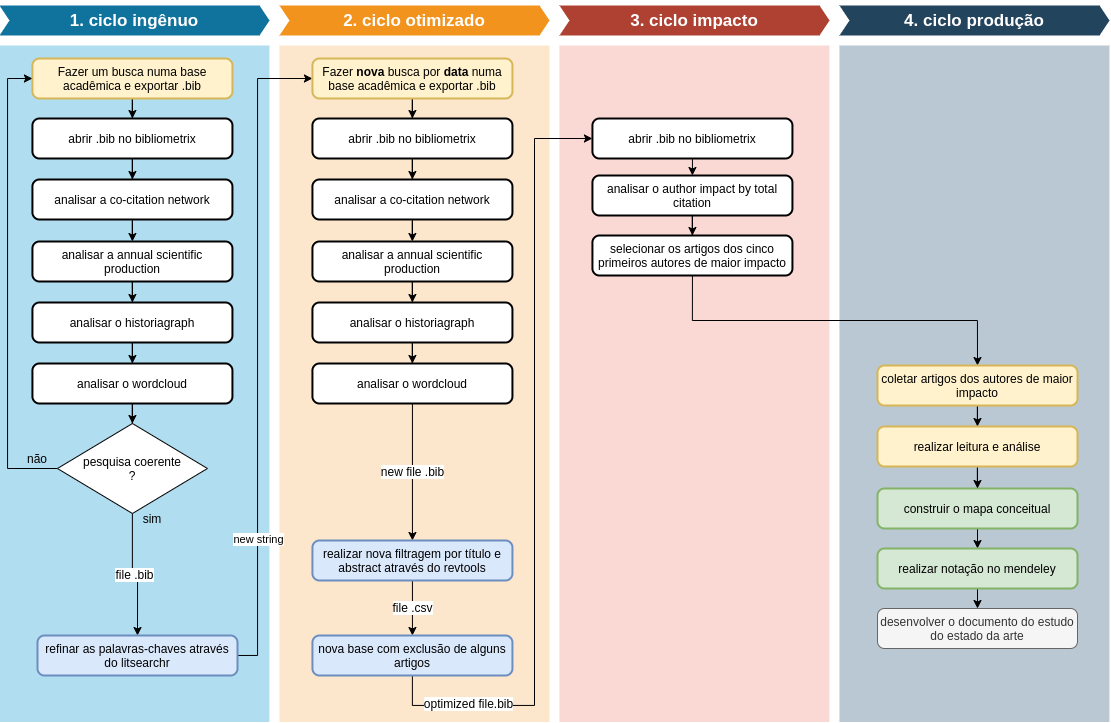
\includegraphics[width=0.6\textwidth]{bili}
    % \caption*{Fonte: Autoria própria.}
    \label{fig:bili}
\end{figure}

\subsection{Fase 1}
\label{sec:fase1}

A primeira fase é denominada de ciclo ingênuo e corresponde a pesquisa inicial feita em uma base acadêmica  de onde foi exportado o arquivo .bib. Através deste arquivo utilizando a ferramenta biblioshiny, fornecida pelo pacote Bibliometrix, foi feita uma análise da rede de co-citação, da produção científica anual e das palavras que aparecem com maior frequência nos artigos. Caso estas informações estejam coerentes com a pesquisa desejada, o pacote litsearchr é utilizado para auxiliar no refinamento da pesquisa através das palavras-chaves. Se o resultado obtido não for satisfatório a busca na base acadêmica deve ser refeita. E, por fim, foi gerada uma nova string que foi utilizada para realizar uma nova busca. 


\subsection{Fase 2}
\label{sec:fase2}

A fase dois é chamada de ciclo otimizado pois, nesta fase foi feita uma nova busca na base acadêmica porém, utilizando as palavras-chaves refinadas. Desta forma, o passo seguinte foi realizar a mesma análise feita no primeiro ciclo e, após está análise foi feita uma filtragem dos artigos utilizando o Revtools. Esta ferramenta permite o pesquisador selecionar os melhores artigos para sua pesquisa através da leitura dos títulos e abstracts. E, então foi exportado um novo arquivo .bib com os dados otimizados para a pesquisa. 

\subsection{Fase 3}
\label{sec:fase3}

Na terceira fase, denominada ciclo impacto, foi feita a análise do impacto do autor utilizando o bibliometrix. E, então foram selecionados os artigos dos cinco primeiros autores de maior impacto.

\subsection{Fase 4}
\label{sec:fase4}

Na última fase, chamada de ciclo produção, é feita a leitura e análise dos artigos selecionados no ciclo anterior e então foi construído um mapa conceitual sobre a pesquisa assim como, todos os artigos selecionados foram armazenados no Mendeley, onde também foram feitas algumas anotações. E, por fim, foi desenvolvida esta documentação com base nestas análises.


% \section{Construção do relatório}
% \label{sec:const}



    \chapter{Estudo do estado da arte}
\label{chap:sota}

\section{Robôs Antropormóficos}
\label{ssec:robos}

Robôs antropormóficos, também conhecidos como humanoides, possuem uma estrutura baseada no corpo humano, com  membros e movimentos que visam uma mobilidade que permita ao robô realizar tarefas diversificadas, principalmente para auxiliar as pessoas em atividades diárias, para o entretenimento e realizar tarefas de risco.

De acordo com \citeonline{Li20211} em comparação com outros tipos de robôs, os humanoides são mais adaptáveis ao ambiente e possuem uma boa habilidade para evitar obstáculos, por isso atraem a atenção de muitos pesquisadores.

Estes robôs movimentam-se e ajustam o seu equilíbrio por meio das suas duas pernas, inclusive em terrenos irregulares. Sendo a habilidade de andar com um bom equilíbrio a sua habilidade mais básica.

Para ter uma boa mobilidade e ser capaz de realizar as tarefas propostas o robô deve possuir uma locomoção rápida e estável, por isso o gerador de trajetórias e o controlador são projetados visando uma locomoção rápida, flexível e robusta. Portanto, são estes os principais desafios no desenvolvimento deste tipo de robô.


%/todo: inserir as outras referencias

\subsection{Definição}
\label{ssec:defi}

Os robôs antropormóficos, também conhecidos como humanoides, são robôs que possuem atributos semelhantes a forma humana como cabeça, braços e pernas. São robôs bípedes, ou seja, que se locomovem sobre os dois pés.

\subsection{Componentes principais}
\label{ssec:comp}

A percepção visual é fundamental para a maioria dos sistemas autônomos que operam em ambientes repletos de obstáculos e para realizar uma série de tarefas essenciais como interagir com o humano, manipular e rastrear objetos. \cite{Joseph2018} 

\citeonline{Chatterjee2017603} aponta que os robôs domésticos utilizam da Inteligência Artificial para possuir habilidades como reconhecimento de voz, reconhecimento facial humano, emoção, entre outros.

E, para garantir que o robô alcance uma locomoção estável e rápida deve-se atentar-se ao projeto da estrutura cinemática do robô e a alguns objetivos do design para melhorar a dinâmica dos membros do robô.\cite{Buschmann2009141}



% \subsection{Tabela Comparativa}
% \label{ssec:tabela}

%/todo: falar sobre a tabela comparativa

%******************************************************************


% \section{Revisão bibliográfica}
% \label{sec:biblio}

% \subsection{Rede de citação}
% \label{ssec:rede}

% \subsection{Principais autores}
% \label{ssec:autor}

%/todo: falar sobre a revisão bibliográfica

%******************************************************************

\section{Modelos de robôs bípedes}
\label{sec:modelos}

Nesta seção serão abordadas as principais características de alguns modelos de robôs humanoides comumente utilizados por pesquisadores para realizar estudos sobre a locomoção bípede.

\subsection{Robô NAO}
\label{ssec:nao}

O NAO (Figura \ref{fig:nao}) é um robô desenvolvido pela SoftBank Robotics muito utilizado para pesquisas e educação. Originalmente, ele foi criado pela Aldebaran Robotics para ser um companheiro doméstico. Dentre as suas principais aplicações estão a sua utilização como assistente em empresas e institutos de saúde. Este robô utiliza um framework específico conhecido como NAOqios, o qual utiliza Python ou C++.  

O NAO possui 58cm de altura, duas câmera 2D para reconhecer objetos e pessoas, é capaz de se comunicar em diversas línguas por meio dos seus quatro microfones e speakers. O robô também dispõe de sete sensores de toque localizados na sua cabeça, nas suas mãos e pés, sonares e uma IMU para reconhecer seu ambiente e se localizar no espaço. Ele apresenta um total de 25 graus de liberdade o que permite que ele se movimente e se adapte no ambiente.

\begin{figure} [H]	
    \centering
    \caption{Robô NAO}
    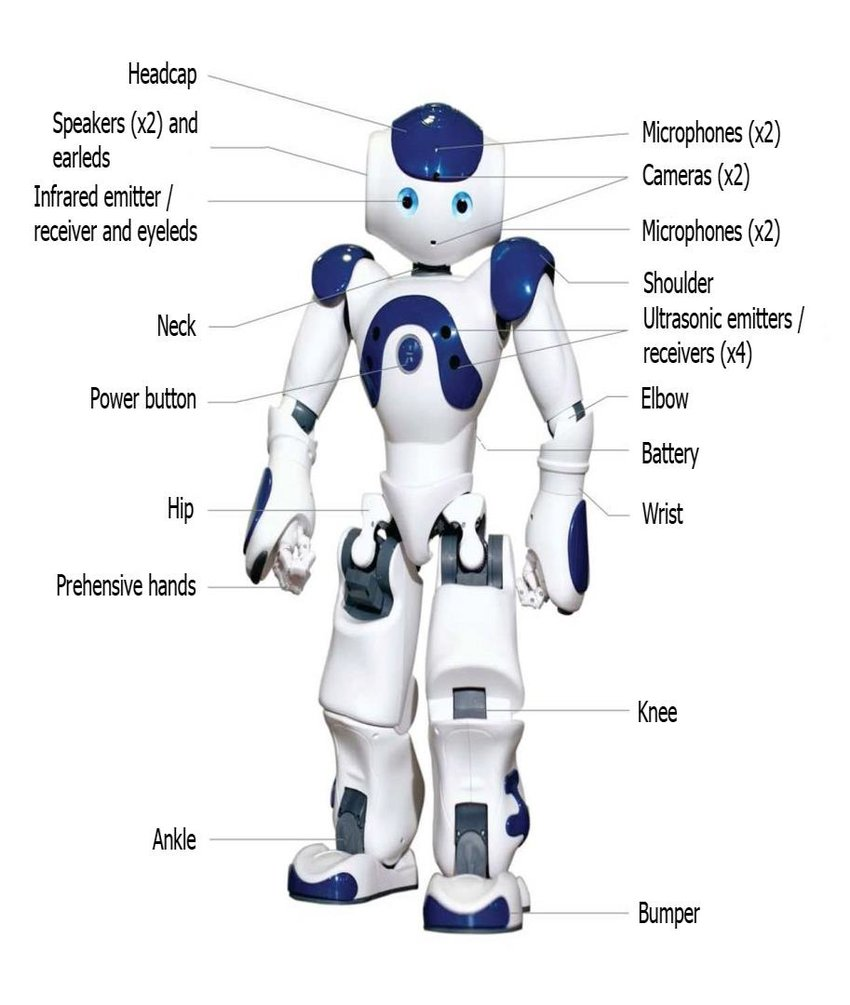
\includegraphics[width=0.45\textwidth]{nao}
    \caption*{Fonte: \cite{NAOxx}.}
    \label{fig:nao}
\end{figure}

\subsection{Robô DARWIN-OP}
\label{ssec:darwin}

O Darwin-OP (Dynamic Anthropomorphic Robot with Intelligence-Open Platform)  é um pequeno humanoide desenvolvido pela Robotis. Ele tem 20 graus de liberdade e pesa 2.9kg, possui uma camera HD, giroscópio, acelerômetro e um microfone stereo. O Darwin é capaz de andar, falar e dançar sendo bastante utilizado por pesquisadores e programadores.

\begin{figure} [H]
    \centering
    \caption{Robô Darwin-OP}
    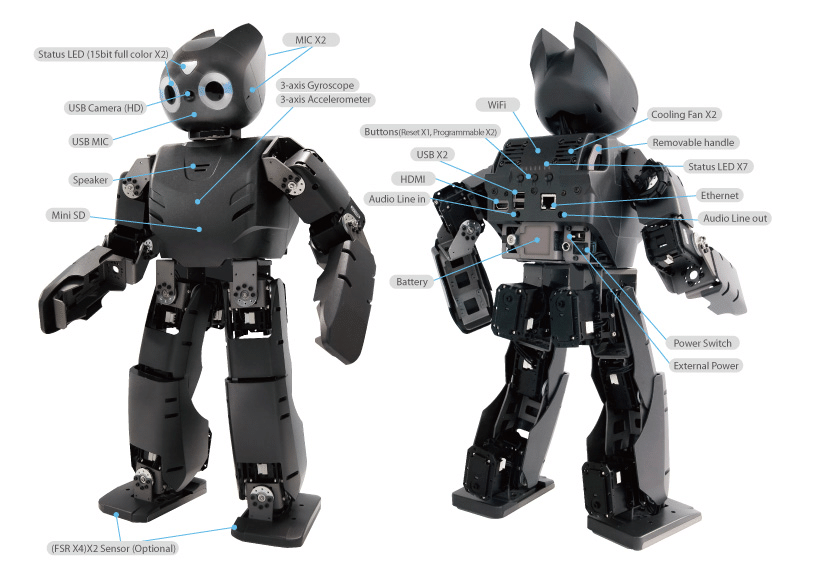
\includegraphics[width=0.65\textwidth]{darwin}
    \caption*{Fonte: \cite{DARWINxx}.}
    \label{fig:darwin}
\end{figure}

\subsection{Robô LOLA}
\label{ssec:lola}

O Lola é um robô humanoide desenvolvido na Universidade Técnica de Munich (TUM) e financiado pela Fundação de pesquisa alemã (DFG), utilizado em pesquisas sobre a dinâmica e aspectos de controle da locomoção bípede. A versão do Lola ilustrada na Figura \ref{fig:lola} possui 24 graus de liberdade, uma altura de 180cm e pesa aproximadamente 60kg. O seu design foi projetado para possuir pouco peso, uma rigidez efetiva alta, pernas com uma inércia baixa e o centro de gravidade alto. Com relação aos sensores utilizados pelo robô, o Lola possui enconders nos eixos dos seus motores e sensores de força/torque (FTS) customizados em seus pés, apresenta uma IMU em seu torso e uma câmera Intel RealSense em sua cabeça. É um robô versátil, com um design projetado para demonstrar uma caminhada bípede rápida.

\begin{figure} [H]
    \centering
    \caption{Robô LOLA}
    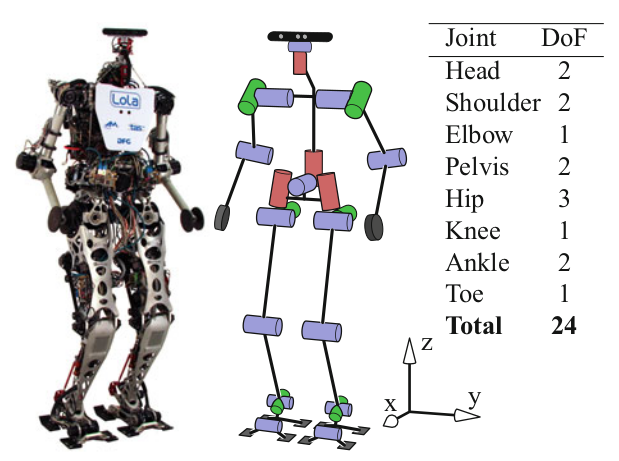
\includegraphics[width=0.6\textwidth]{lola}
    \caption*{Fonte: \cite{LOLAxx}.}
    \label{fig:lola}
\end{figure}

\subsection{Robô HUBO 2}
\label{ssec:hubo}

O HUBO 2 foi desenvolvido no laboratório HUBO no KAIST (Korean Advanced Institute os Science and Technology), na Coréia do Sul. Ele possui 125cm, pesa 45kg e possui 40 graus de liberdade. O seu design tinha como objetivo ser bem leve, o que permitiu que o HUBO 2 fosse capaz de correr em uma velocidade de 3.6 km/h. O seu sistema de percepção é composto por câmeras, sensores de inércia, inclinação e  força/torque. O seu grande diferencial em relação a outros robôs bípedes é a capacidade de utilizar uma marcha com pernas esticadas.

\begin{figure} [H]
    \centering
    \caption{Robô HUBO 2}
    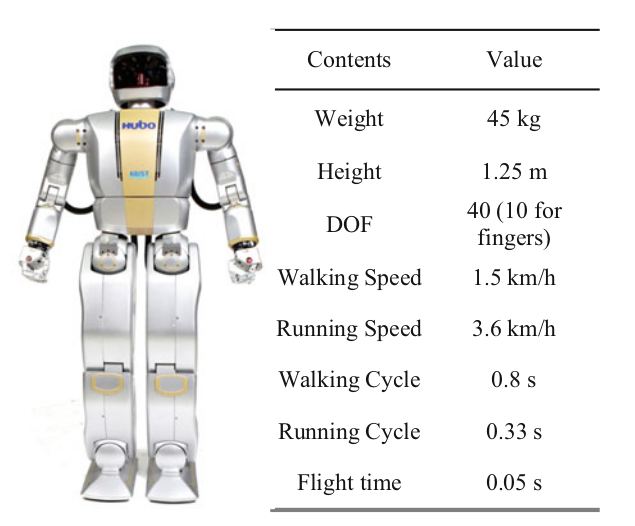
\includegraphics[width=0.5\textwidth]{hubo2}
    \caption*{Fonte: \cite{HUBOxx}.}
    \label{fig:hubo2}
\end{figure}


\section{Estudo das funcionalidades e mecânismos}
\label{sec:robos}

Nesta seção serão apresentadas as principais características dos sistemas de percepção e controle dos robôs antropormóficos, assim como da estrutura mecânica destes robôs. Estes são quesitos de extrema importância no desenvolvimento destes robôs pois influênciam na eficiência do seu sistema.

\subsection{Percepção}
\label{ssec:percepcao}

Os sensores comumente usados nos robôs humanoides podem ser classificados em dois grupos (Figura \ref{fig:sensors}), os sensores proprioceptivos são utilizados para medir os estados de cada junta e do corpo do robô e os sensores exteroceptivos são utilizados para obter informações do ambiente \cite{He2020}.

Os sensores internos são utilizados para medir o estado do robô, como ângulos, velocidades e torques das juntas. Para detectar informações da postura do robô, utiliza-se os sensores IMU, incluindo acelerômetros e giroscópios. Enquanto, a interação entre o robô e o ambiente podem ser detectadas por meio de sensores táteis e de força/torque. E, as câmeras e sensores de alcance medem e estimam as informações do ambiente ao redor do robô \cite{Ambarish20181}.

\begin{figure} [H]
    \centering
    \caption{Classificação dos sensores}
    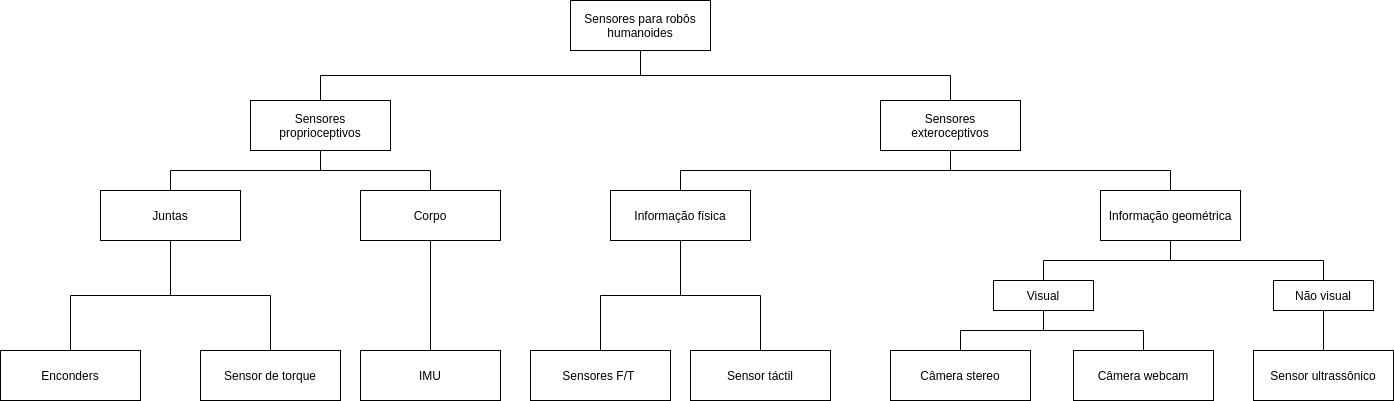
\includegraphics[width=\textwidth]{sensores}
    % \caption*{Fonte: Autoria própria.}
    \label{fig:sensors}
\end{figure}

O sistema de sensores do LOLA, por exemplo, de acordo com \citeonline{Buschmann2009141},  é otimizado para qualidade de sinal e largura de banda. Sensores angulares absolutos nos eixos de saída de todas as juntas compensam as elasticidades e não linearidades, permitindo que o robô (teoricamente) comece a partir de posições arbitrárias. Dois sensores de força / torque de seis eixos feitos sob medida são fortemente integrados à estrutura do pé. Com um peso total de 395g, o sensor inclui uma proteção contra sobrecarga. A unidade de medição inercial (IMU) estima a orientação e as velocidades angulares da parte superior do corpo. foi escolhida IMU de alta precisão com giroscópios de fibra ótica e acelerômetros MEMS, visto que a precisão e a qualidade do sinal do IMU afetam consideravelmente o desempenho do controlador de estabilização

%/todo: tabela com estes dados

Já no projeto desevolvido por \citeonline{Kien2017} quatro sensores ultrassônicos, dois em cada perna, são usados para feedback da posição para caminhar e girar. O acelerômetro é usado para medir o ângulo de inclinação e para detectar a queda instantânea do robô. Sensores Resistivos de Força (FSR) são usados para determinar o centro de pressão (COP), que por sua vez é usado para calcular o ZMP do robô.

%/todo: tabela com estes dados

\subsection{Mecânismos}
\label{ssec:mec}

Um robô humanoide tem o formato do corpo semelhante ao de um corpo humano e tem como base a literatura sobre a análise e coordenação da marcha humana. Eles possuem um grande número de graus de liberdade (DOF), para serem capazes de realizar um movimento bípede semelhante ao humano. Para que este movimento seja mais natural e flexível, segundo \citeonline{Buschmann2009141}, recomenda-se considerar uma configuração redundante com DOFs adicionais.

Para melhorar a dinâmica das pernas do robô deve-se garantir uma rigidez mecânica suficiente, centro de massa alto e baixos momentos de inércia dos elos das pernas.

O objetivo básico do projeto de um robô humanoide, é, portanto, equilibrar a rigidez estrutural e o desempenho do atuador com a leveza dos componentes mecânicos.
A estrutura mecânica do Lola, por exemplo, é caracterizado pelo design leve e consistente com alta rigidez efetiva \ref{ssec:lola}. São utilizados servo atuadores leves e a inércia resultante das pernas é minimizada por um design sofisticado da estrutura e mecanismos de acionamento, resultando em um comportamento de aceleração superior.

%/todo: abordar a estrutura de um robô menor
%/todo: inserir ilustrações

\subsection{Controle}
\label{ssec:control}

A figura \ref{fig:steps-control} ilustra os passos necessários para o controle da caminhada de um robô humanoide, onde a primeira etapa deste processo é o planejamento dos passos o qual é feito através do ajuste de alguns parâmetros de forma que o robô realize os movimentos de acordo com as fases de suporte dos pés ilustradas na figura \ref{fig:support-phases}.


\begin{figure} [H]
    \centering
    \caption{Elementos para o desenvolvimento do controlador de caminhada}
    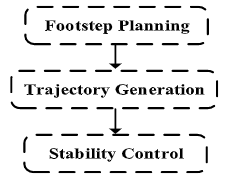
\includegraphics[width=0.3\textwidth]{walk-control}
    \caption*{Fonte: \cite{Kashyap2021306}.}
    \label{fig:steps-control}
\end{figure}


\begin{figure} [H]
    \centering
    \caption{Diferentes fases de suporte dos pés durante a locomoção de robôs humanoides}
    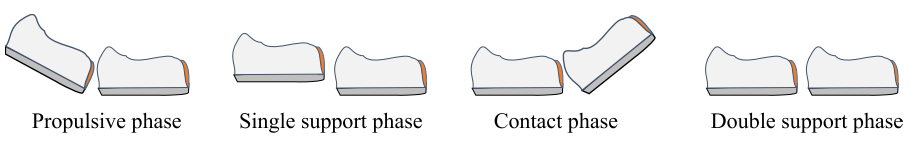
\includegraphics[width=0.8\textwidth]{support-phases}
    \caption*{Fonte: \cite{Kashyap2021306}.}
    \label{fig:support-phases}
\end{figure}

Existem basicamente dois tipos de marchas observadas em sistemas com pernas:  estaticamente estável e  dinâmicamente estável. Se o passo do robô permite que a projeção do seu centro de massa permaneça suficientemente dentro do polígono de suporte, projetado pelo pé do robô, então é estaticamente estável. E, se a projeção ocasionalmente sai do polígono de suporte , não deixando o robô cair ou tombar, então o sistema é dinâmicamente estável \cite{Ambarish20181}.

Existem quatro modelos que são frequentemente utilizados como representação aproximada do robô bípede (Figura \ref{fig:modelos-pendulos}). O Modelo do Pêndulo Invertido Linear (LIPM) considera que toda a massa do robô está concentrada em um ponto movendo-se em uma altura constante e assume que as pernas não possuem peso,  este modelo foi amplamente aplicado em diversas pesquisas como  por \citeonline{Kashyap2021306}, que utilizaram a técnica de optimização por enxame de partículas (PSO) para refinar o controlador PID convencional e bastante estudado e aplicado por \citeonline{Kajit201}.

\begin{figure} [H]
    \centering
    \caption{Modelos frequentemente utilizados como representações dos robôs bípedes}
    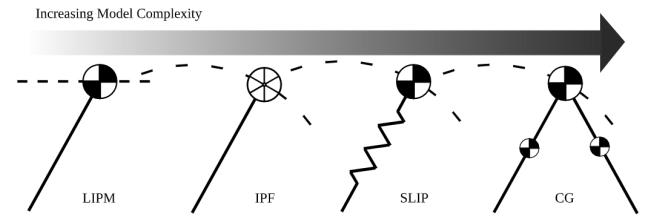
\includegraphics[width=0.8\textwidth]{modelos-pendulos}
    \caption*{Fonte: \cite{Grizzle20141955}.}
    \label{fig:modelos-pendulos}
\end{figure}

Um outro modelo é o Pêndulo Invertido com Volante (IPF) que não considera a altura constante e adiciona um volante para contabilizar o momento angular interno. O Pêndulo Invertido com Mola (SLIP) adiciona uma mola para modelar as pernas do robô como um pula-pula sem massa. E o Compass -Gait Biped (CG) que trata o robô como um pêndulo duplo com massas concentradas no centro de massa e nas pernas oscilantes \cite{Grizzle20141955}. Ao utilizar um modelo de robô reduzido \citeonline{Wahrmann20171471}, por exemplo, foi capaz de implementar a estratégia no controle em tempo real tornando o robô mais robusto contra erros de percepção e de superfícies irregulares. 

Posteriormente, deve-se implementar um gerador de trajetórias, o qual gera algum tipo de movimento considerando o deslocamento do Centro de Massa (COM) e do Ponto de Momento Zero (ZMP) assim como, a descrição da cinemática inversa. Desta forma, os ângulos das juntas do robô são obtidas. E, então é necessário um controlador para estabilizar estes ângulos  para garantir que o robô permaneça em pé e realize todas as tarefas sem cair. \cite{Kashyap2021306}

\citeonline{Kasaei2018743} apresenta uma estrutura de um controlador com um loop fechado baseada no método Central Pattern Generator (CPG) que propõem um modelo de controle inspirado nas características biológicas (Figura \ref{fig:arquitetura-nao}). Desta forma, este método tenta produzir um caminhar estável através de padrões rítmicos em relação a movimentação dos seus membros. Este teste foi realizado em um robô NAO simulado com a proposta de gerar uma movimentação estável e rápida.

\begin{figure} [H]
    \centering
    \caption{Arquitetura geral do gerador de passos}
    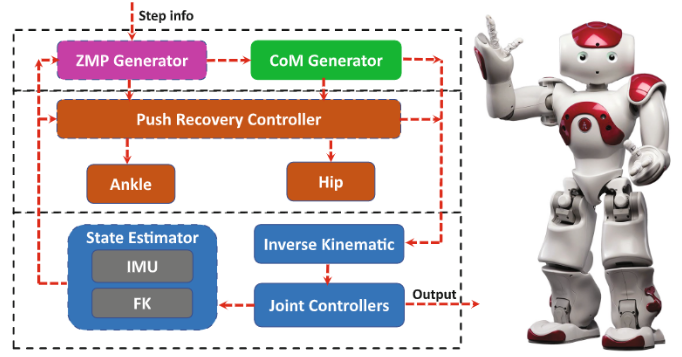
\includegraphics[width=0.4\textwidth]{arquiteturaNAO}
    \caption*{Fonte: \cite{Kasaei2018743}}
    \label{fig:arquitetura-nao}
\end{figure}

Em sua pesquisa \citeonline{Joe2019} implementam um framework de controle do equilíbrio que estabiliza os passos do robô em relação aos distúrbios. O controlador de equilíbrio é formado pelos controladores de orientação dos pés, comprimento da perna e ZMP. Os testes foram realizados no robô DRC-HUBO+ modificado. E, o framework proposto apresentou bons resultados permitindo que o robô se deslocasse de forma estável mantendo a postura desejada em terrenos irregulares.


\begin{figure} [H]
    \centering
    \caption{Visão geral do fluxo de informações do framework de controle de equilíbrio proposto}
    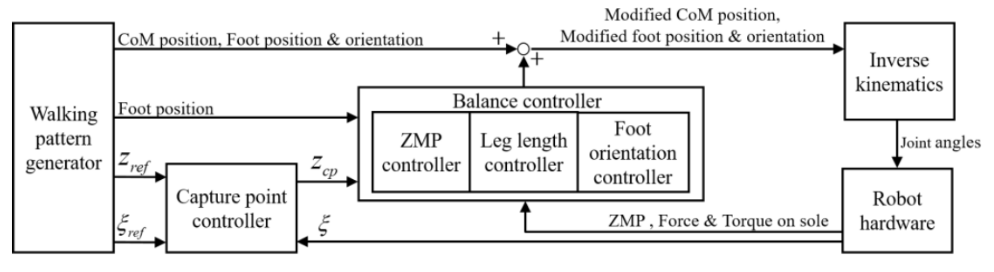
\includegraphics[width=0.8\textwidth]{controlador}
    \caption*{Fonte: \cite{Joe2019}}
    \label{fig:framework-control}
\end{figure}


O projeto de controle para sistemas subactuados são mais difícies devido a quantidade de graus de liberdades controláveis ser menor que a real quantidade de grau de liberdade do sistema. \citeonline{Gupta2017607} abordam outras estratégias de controle desenvolvidas para robôs subactuados como virtual constraints, HZD (Hybrid Zero Dynamics), Pointcaré map.



%******************************************************************

% \section{Mapa conceitual do estudo}
% \label{sec:mapa}



%******************************************************************

% \section{Organização e compartilhamento dos dados}
% \label{sec:org}


%******************************************************************







    % \chapter{Conclusão}
\label{chap:conc}

Chegou a hora de apresentar o apanhado geral sobre o trabalho de
pesquisa feito, no qual s\~ao sintetizadas uma s\'erie de
reflex\~oes sobre a metodologia usada, sobre os achados e
resultados obtidos, sobre a confirma\c{c}\~ao ou recha\c{c}o da
hip\'otese estabelecida e sobre outros aspectos da pesquisa que
s\~ao importantes para validar o trabalho. Recomenda-se n\~ao
citar outros autores, pois a conclus\~ao \'e do pesquisador.
Por\'em, caso necess\'ario, conv\'em cit\'a-lo(s) nesta parte e
n\~ao na se\c{c}\~ao seguinte chamada \textbf{Conclus\~oes}.


\section{Considerações finais}
\label{sec:consid}

Brevemente comentada no texto acima, nesta se\c{c}\~ao o
pesquisador (i.e. autor principal do trabalho cient\'ifico) deve
apresentar sua opini\~ao com respeito \`a pesquisa e suas
implica\c{c}\~oes. Descrever os impactos (i.e.
tecnol\'ogicos,sociais, econ\^omicos, culturais, ambientais,
políticos, etc.) que a pesquisa causa. N\~ao se recomenda citar
outros autores.


    % include more chapters ...
%
% ----------------------------------------------------------------------------
% Include thesis appendices
    \begin{thesisappendices}
        % Thesis Appendix -------------------------------------------------------

\chapter{Comparativo entre modelos de robôs antropormóficos}
\label{Append:comp}

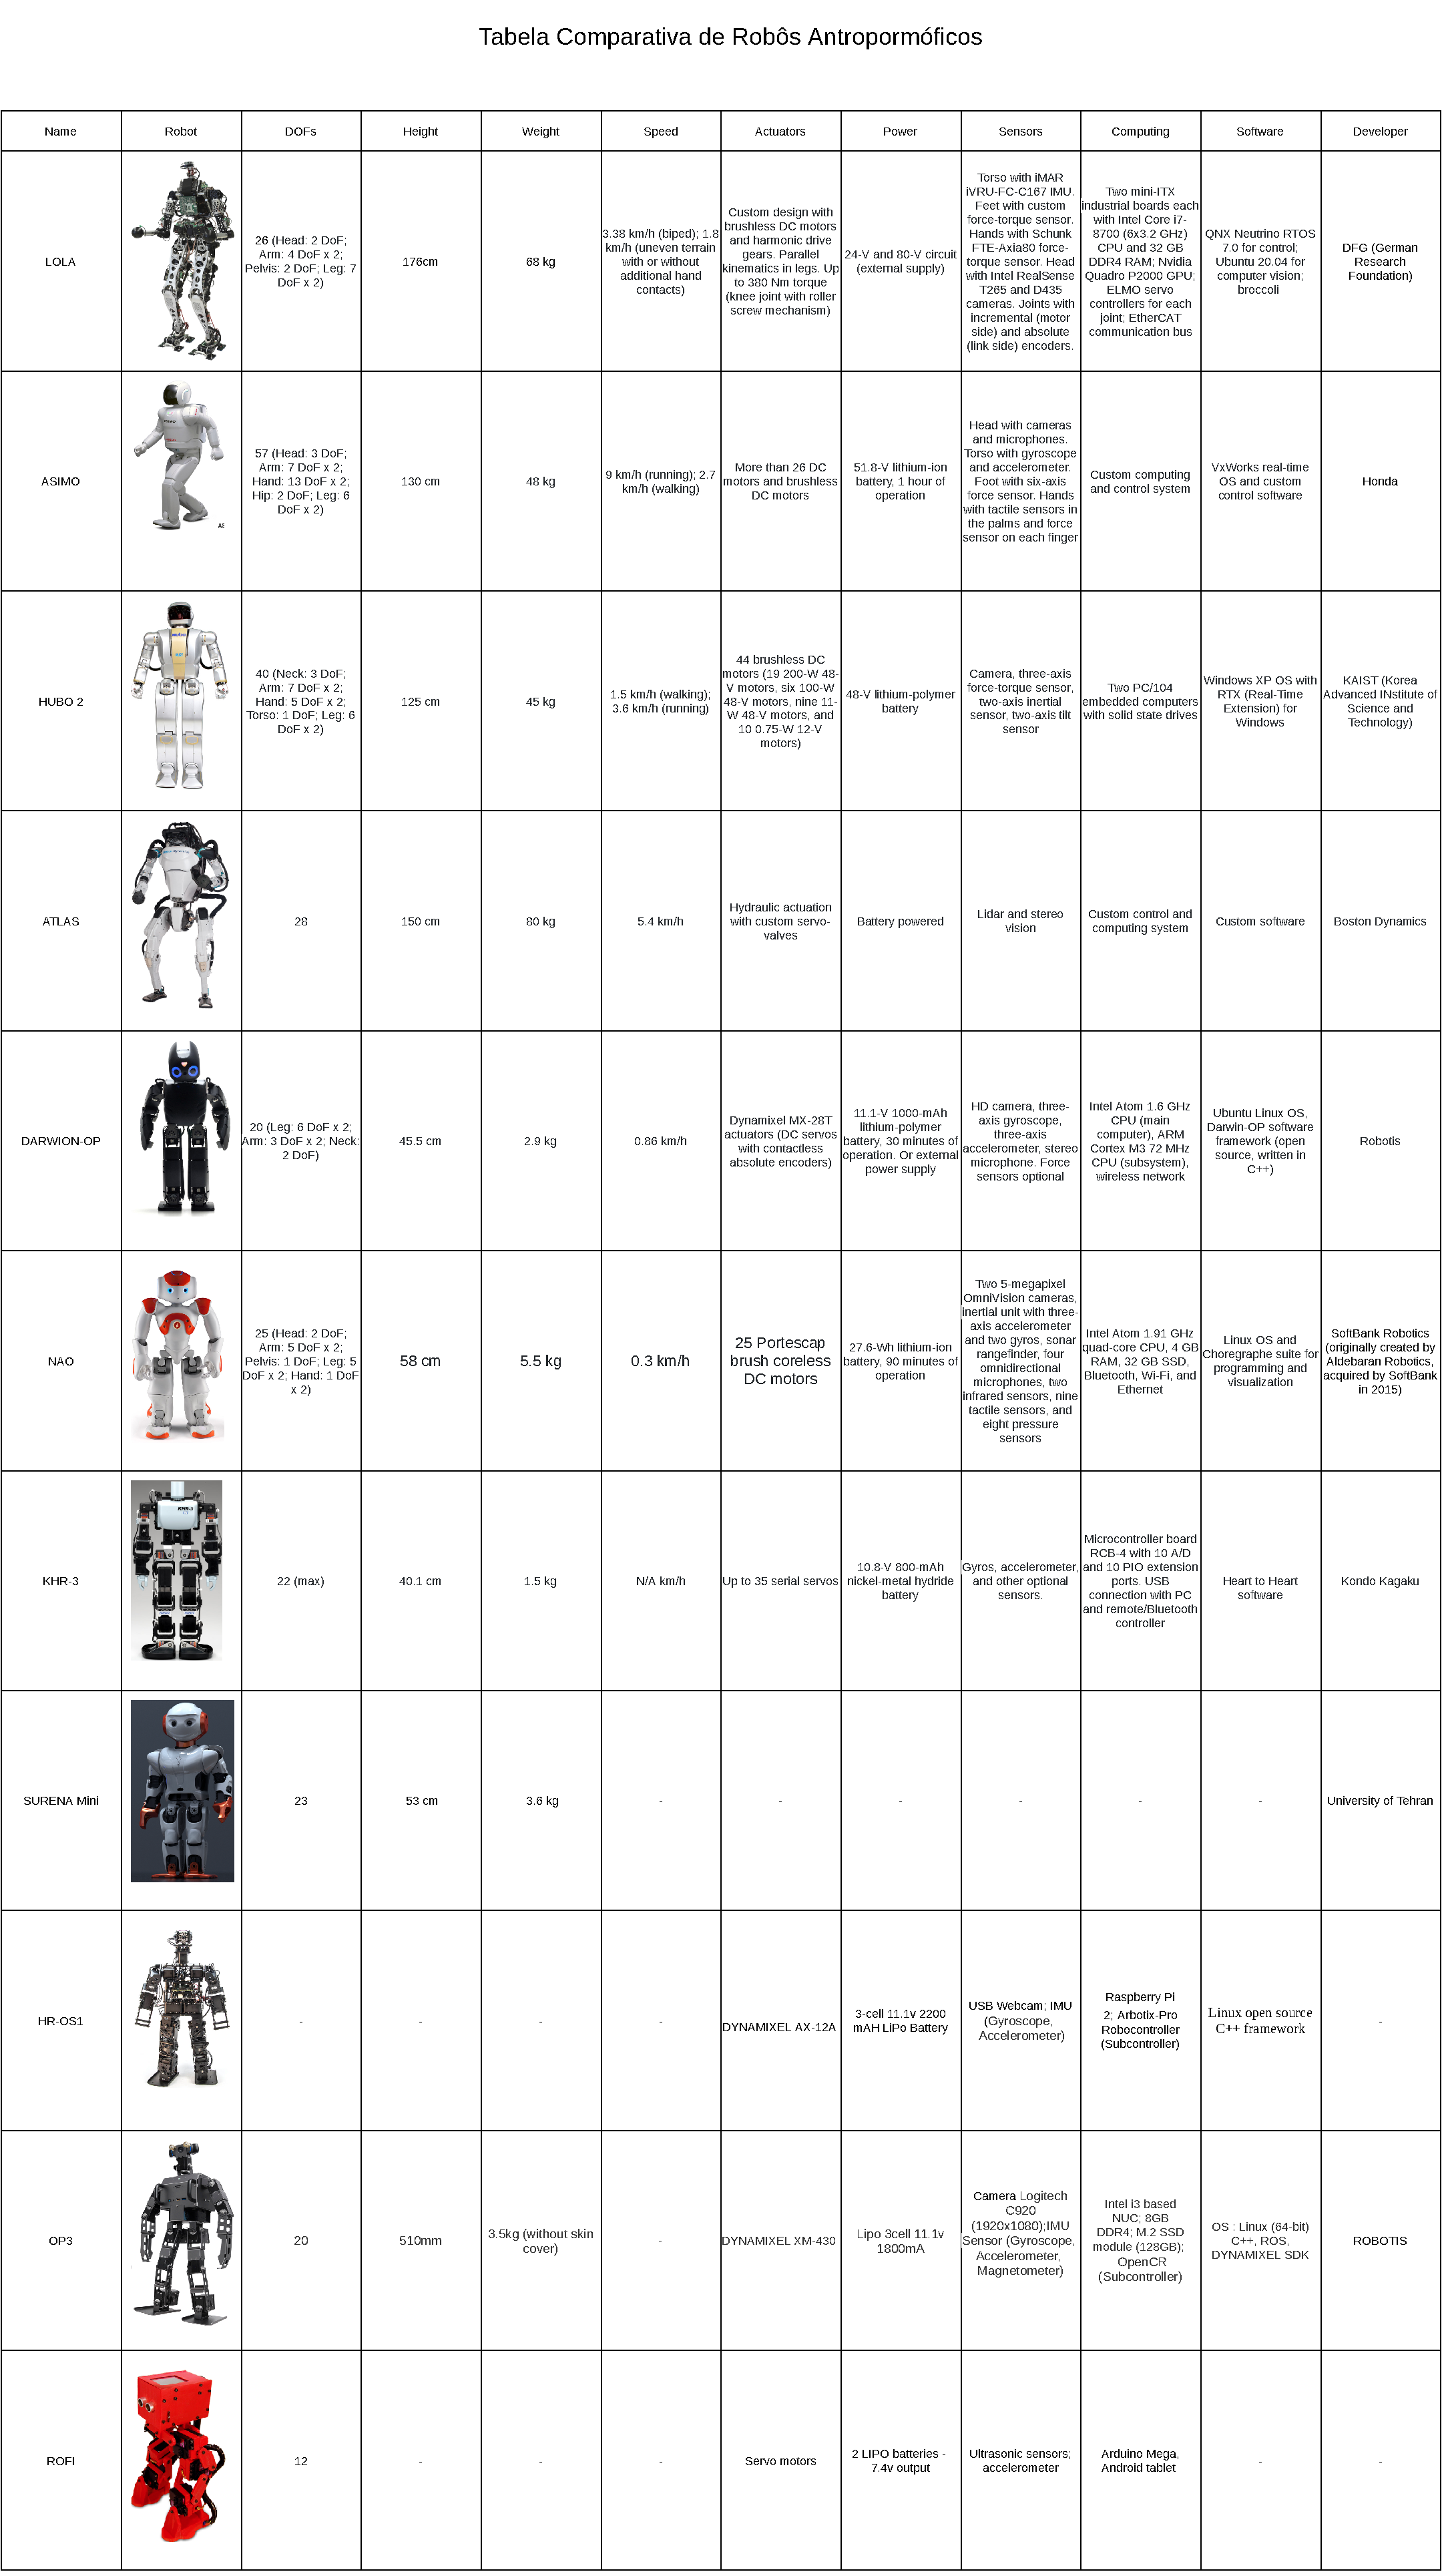
\includepdf[pages={1}]{Appendices/comparativo.pdf}



        % % Thesis Appendix -------------------------------------------------------

\chapter{Diagramas eletro-eletrônicos}
\label{Append:diagele}



        %% Thesis Appendix -------------------------------------------------------

\chapter{Logbook}
\label{Append:log}



    \end{thesisappendices}
%
% ----------------------------------------------------------------------------
% Configurar as referencias bibliograficas
	\renewcommand\bibname{Referências}
    \addcontentsline{toc}{chapter}{Referências}
    \bibliography{References/referencias}
%
% ----------------------------------------------------------------------------
% Finishing him
    \include{Others/ultimafolha}
\end{document}
%
% -------------------------------------------------------------------------------
% Aqui termina a formatação para o documento.
% In God We Trust. All Other Bring Data. 
%
% -------------------------------------------------------------------------------